% Copyright 2004 by Till Tantau <tantau@users.sourceforge.net>.
%
% In principle, this file can be redistributed and/or modified under
% the terms of the GNU Public License, version 2.
%
% However, this file is supposed to be a template to be modified
% for your own needs. For this reason, if you use this file as a
% template and not specifically distribute it as part of a another
% package/program, I grant the extra permission to freely copy and
% modify this file as you see fit and even to delete this copyright
% notice. 
\documentclass{beamer}
\usepackage{bbm}
\usepackage{lipsum}
\usepackage{enumitem}
\usepackage{pifont}
\usepackage{tikz}
\usepackage{lmodern}
\usepackage{commath}
\usepackage{bbm} %package for using the bbm fonts in math environment
\usetikzlibrary{calc}
\usepackage{xparse} 
\usetikzlibrary{calc}
\logo{\color{red}\rule{.5cm}{.5cm}}
\newcommand{\btVFill}{\vskip0pt plus 1filll}
\usepackage{afterpage}
\usepackage{xcolor}
\usepackage{tcolorbox}

%\usepackage{xcolor}
%\usepackage{tikz}
%\usetikzlibrary{shadows}
\newlength{\tmpShadow}
\newcommand{\MyShadow}[2]{%
	\settowidth{\tmpShadow}{#1}
	\addtolength{\tmpShadow}{.1em}
	\raisebox{-0.25ex}{\textcolor{gray!70}{#1}}%
	\kern-\tmpShadow%
	\textcolor{#2}{#1}%
}


\tikzset{
	invisible/.style={opacity=0,text opacity=0},
	visible on/.style={alt=#1{}{invisible}},
	alt/.code args={<#1>#2#3}{%
		\alt<#1>{\pgfkeysalso{#2}}{\pgfkeysalso{#3}} 
	},
}
\tikzset{
	background fill/.style={fill=#1},
	background fill/.default={white},
	fill on/.style={alt=#1{}{background fill}},
}
\tikzset{
	background draw/.style={draw=#1},
	background draw/.default={white},
	draw on/.style={alt=#1{}{background draw}},
}
\tikzset{
	background filldraw/.style args={#1 filled by #2}{draw=#1, fill=#2},
	background filldraw/.default=white filled by white,
	filldraw on/.style={alt=#1{}{background filldraw}},
}
\tikzset{highlighting/.style={
		append after command={
			\pgfextra{
				\path[rounded corners,
				background draw=red,
				draw on=<#1>,
				overlay] ($(\tikzlastnode.south west)+(-0.015,-0.1)$) % to have some offset
				rectangle ($(\tikzlastnode.north east)+(0.015,0.07)$);
			}   
		}
	}
}
\NewDocumentCommand{\highlight}{r<> m}{%
	\tikz[baseline=(A.base)] 
	\node[highlighting=#1,
	inner sep=0pt] (A) {#2};%
}

%\newcommand*{\MyShadowBullet}{\tikz \draw [baseline, fill=blue,draw=blue,circular drop shadow] circle (2pt);}
%\newcommand*{\MyBallBullet}{\tikz \draw [baseline, ball color=red, draw=red] circle (2pt);}

\newcommand{\nologo}{\setbeamertemplate{logo}{}} % command to set the logo to nothing
\usepackage{multicol}
\newcommand\tab[1][1cm]{\hspace*{#1}}

%gets rid of bottom navigation bars
%\setbeamertemplate{footline}[frame number]{}
%gets rid of bottom navigation symbols
\setbeamertemplate{navigation symbols}{}
%gets rid of footer
%will override 'frame number' instruction above
%comment out to revert to previous/default definitions
%\setbeamertemplate{footline}{}

\newcounter{mycounter}  
\newenvironment{noindlist}
{\begin{list}{}{\usecounter{mycounter} \labelsep=0em \labelwidth=0em \leftmargin=0em \itemindent=0em}}
	{\end{list}}

% There are many different themes available for Beamer. A comprehensive
% list with examples is given here:
% http://deic.uab.es/~iblanes/beamer_gallery/index_by_theme.html
% You can uncomment the themes below if you would like to use a different
% one:
%\usetheme{AnnArbor}
%\usetheme{Antibes}
%\usetheme{Bergen}
%\usetheme{Berkeley}
%\usetheme{Berlin}
%\usetheme{Boadilla}
%\usetheme{boxes}
%\usetheme{CambridgeUS}
%\usetheme{Copenhagen}
%\usetheme{Darmstadt}
%\usetheme{default}
%\usetheme{Frankfurt}
%\usetheme{Goettingen}
%\usetheme{Hannover}
%\usetheme{Ilmenau}
%\usetheme{JuanLesPins}
%\usetheme{Luebeck}
\usetheme{Madrid}
%\usetheme{Malmoe}
%\usetheme{Marburg}
%\usetheme{Montpellier}
%\usetheme{PaloAlto}
%\usetheme{Pittsburgh}
%\usetheme{Rochester}
%\usetheme{Singapore}
%\usetheme{Szeged}
%\usetheme{Warsaw}

%\setbeamercolor{normal text}{fg=white,bg=black!90}
%\setbeamercolor{structure}{fg=blue!80}
%\setbeamercolor{alerted text}{fg=red!85!black}
%\setbeamercolor{item projected}{use=item,fg=black,bg=item.fg!35}
%\setbeamercolor*{palette primary}{use=structure,fg=structure.fg}
%\setbeamercolor*{palette secondary}{use=structure,fg=structure.fg!95!black}
%\setbeamercolor*{palette tertiary}{use=structure,fg=structure.fg!90!black}
%\setbeamercolor*{palette quaternary}{use=structure,fg=structure.fg!95!black,bg=black!80}
%\setbeamercolor*{framesubtitle}{fg=white}
%\setbeamercolor*{block title}{parent=structure,bg=black!60}
%\setbeamercolor*{block body}{fg=black,bg=blue!10}
%\setbeamercolor*{block title alerted}{parent=alerted text,bg=black!15}
%\setbeamercolor*{block title example}{parent=example text,bg=black!15}


\title{Machine learning methods for path analysis in behavioural neuroscience}

% A subtitle is optional and this may be deleted
%\subtitle{Optional Subtitle}

\author{Avgoustinos~Vouros\inst{1}}
% - Give the names in the same order as the appear in the paper.
% - Use the \inst{?} command only if the authors have different
%   affiliation.

\institute[] % (optional, but mostly needed)
{
  \inst{1}%
  PhD student, \\Department of Computer Science,\\
  University of Sheffield\\
  \vspace{5mm}
  \noindent Supervised by Prof Eleni Vasilaki
  %\and
  %\inst{2}%
  %Department of Theoretical Philosophy\\
  %University of Elsewhere
}

\date{} %removes the date
% - Use the \inst command only if there are several affiliations.
% - Keep it simple, no one is interested in your street address.

%\date{Conference Name, 2013}
% - Either use conference name or its abbreviation.
% - Not really informative to the audience, more for people (including
%   yourself) who are reading the slides online

%\subject{Theoretical Computer Science}
% This is only inserted into the PDF information catalog. Can be left
% out. 

% If you have a file called "university-logo-filename.xxx", where xxx
% is a graphic format that can be processed by latex or pdflatex,
% resp., then you can add a logo as follows:

\pgfdeclareimage[height=1cm]{university-logo}{university-logo}
\logo{\pgfuseimage{university-logo}}

% Delete this, if you do not want the table of contents to pop up at
% the beginning of each subsection:
\AtBeginSubsection[]
{
  \begin{frame}<beamer>{Outline}
    \tableofcontents[]
  \end{frame}
}

% Let's get started
\begin{document}

\begin{frame}
  \titlepage
\end{frame}

%\begin{frame}{Acknowledgements}
%	Original slides created by: 
%	\begin{itemize}
%		\item Eleni Vasilaki (Prof)
%		\item Tiago V. Gehring (PhD)
%	\end{itemize}
%	\vspace{5mm}
%	Revised and modified slides created by:
%	\begin{itemize}
%		\item Avgoustinos Vouros
%	\end{itemize}	
%\end{frame}

%%%%%%%%%%%%%%%%%%%%%%%%%%%%%%%%%%%%%%%%%%%%%%%%%%%%%%%%%

%\begin{frame}{Contents}
%	\begin{itemize}[label={\MyShadow{$\bullet$}{black!80}}]
%		\item The story so far...
%		\vspace{3mm}
%		\item Features
%		\vspace{3mm}
%		\begin{itemize}[label={\MyShadow{$\bullet$}{black!80}}]
%			\item Theory
%			\begin{itemize}[label={\MyShadow{$\star$}{black!80}}]
%				\item Regression (quick)
%			\end{itemize}	
%			\vspace{3mm}
%			\item Algorithm
%			\vspace{3mm}
%			\item Tuning
%			\begin{itemize}[label={\MyShadow{$\star$}{black!80}}]
%				\item Gap Statistic
%			\end{itemize}				
%		\end{itemize}
%		\vspace{1mm}
%		\item Ongoing Research
%	\end{itemize}
%\end{frame}


{\nologo


\begin{frame}{Behavioural experiments}
\begin{figure}[H]
	\centering
	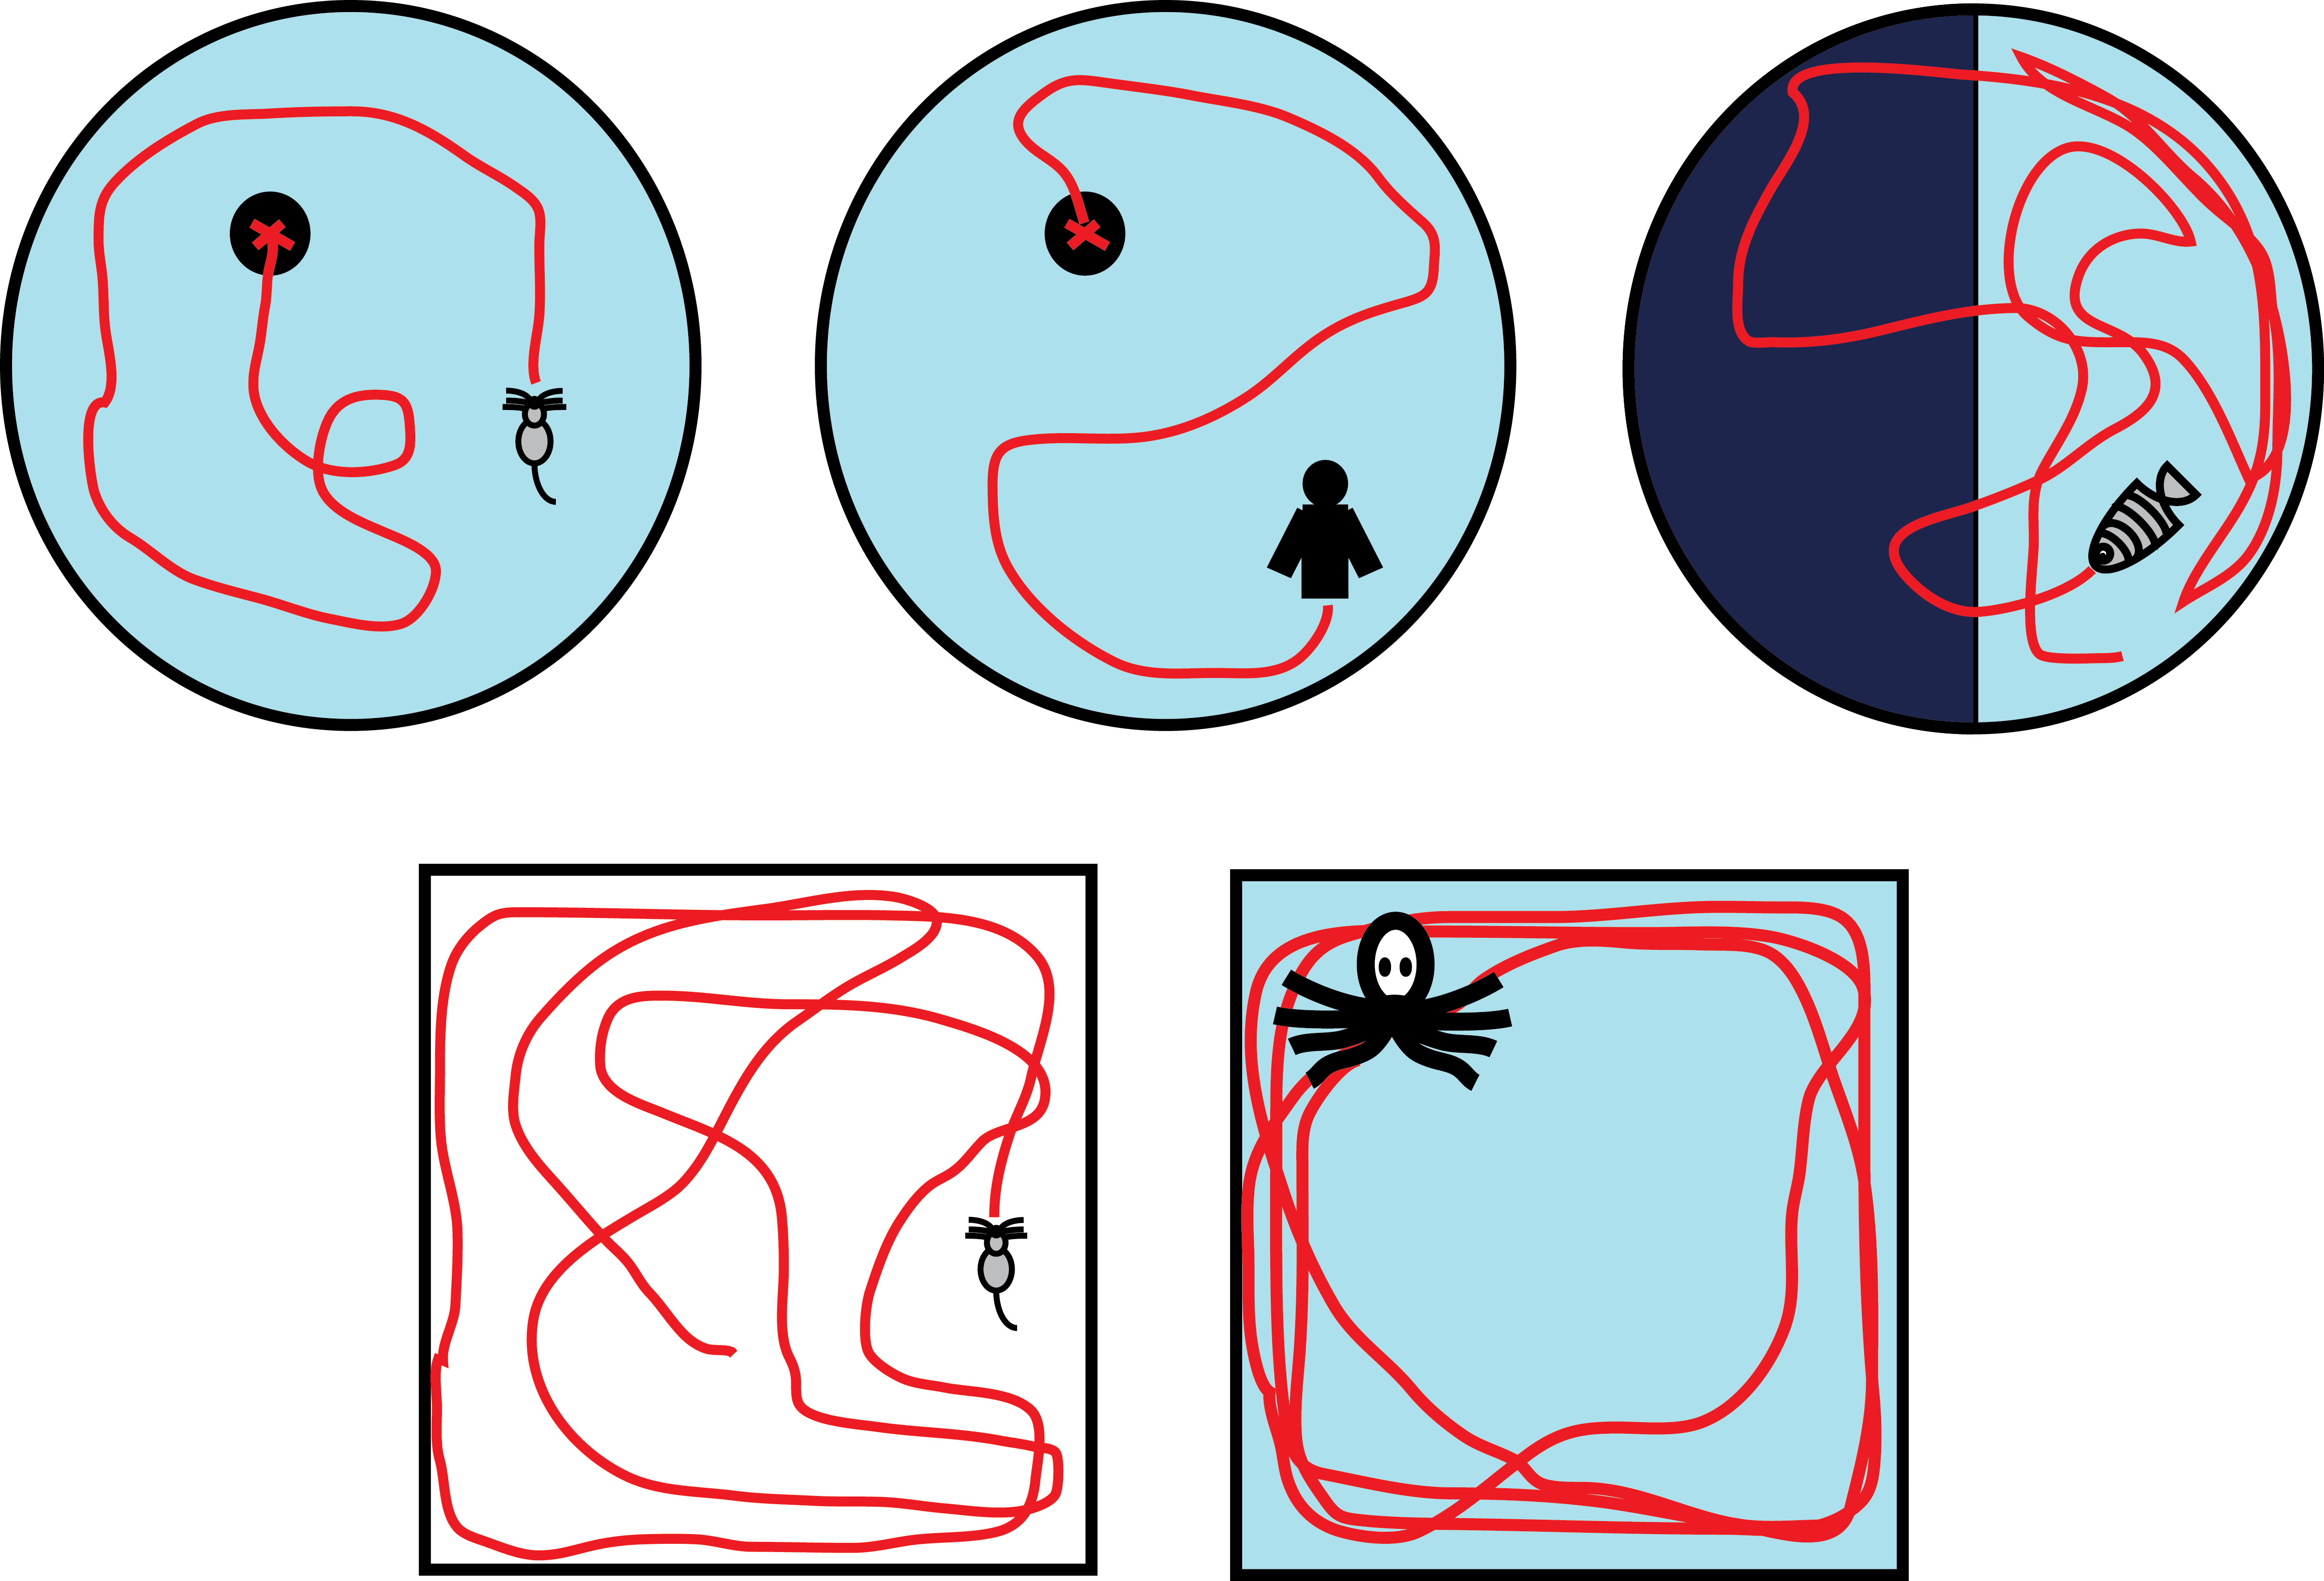
\includegraphics[width=0.9\textwidth]{figures/experiments}
\end{figure}
\end{frame}


\begin{frame}{Behavioural experiments}
\begin{multicols}{2}
	\begin{itemize}[label={\MyShadow{$\bullet$}{blue!80}}, leftmargin=*]
		\item<1-> Collect trajectory/path data.
		\item<2-> Compute various performance measurements.
		
\includegraphics[width=0.30\textwidth]{figures/performance}
		\item<3-> \textbf{Quantify behavioural differences.}
		\uncover<4->{
			\begin{itemize}[label={\MyShadow{$\bullet$}{violet!80}}, leftmargin=*]
				\setlength\itemsep{0.01em}
				\item Machine learning frameworks.
				\item Capture behavioural differences to a greater degree.
			\end{itemize} 
		}
	\end{itemize}
	\columnbreak
	\begin{figure}[H]
		\centering
		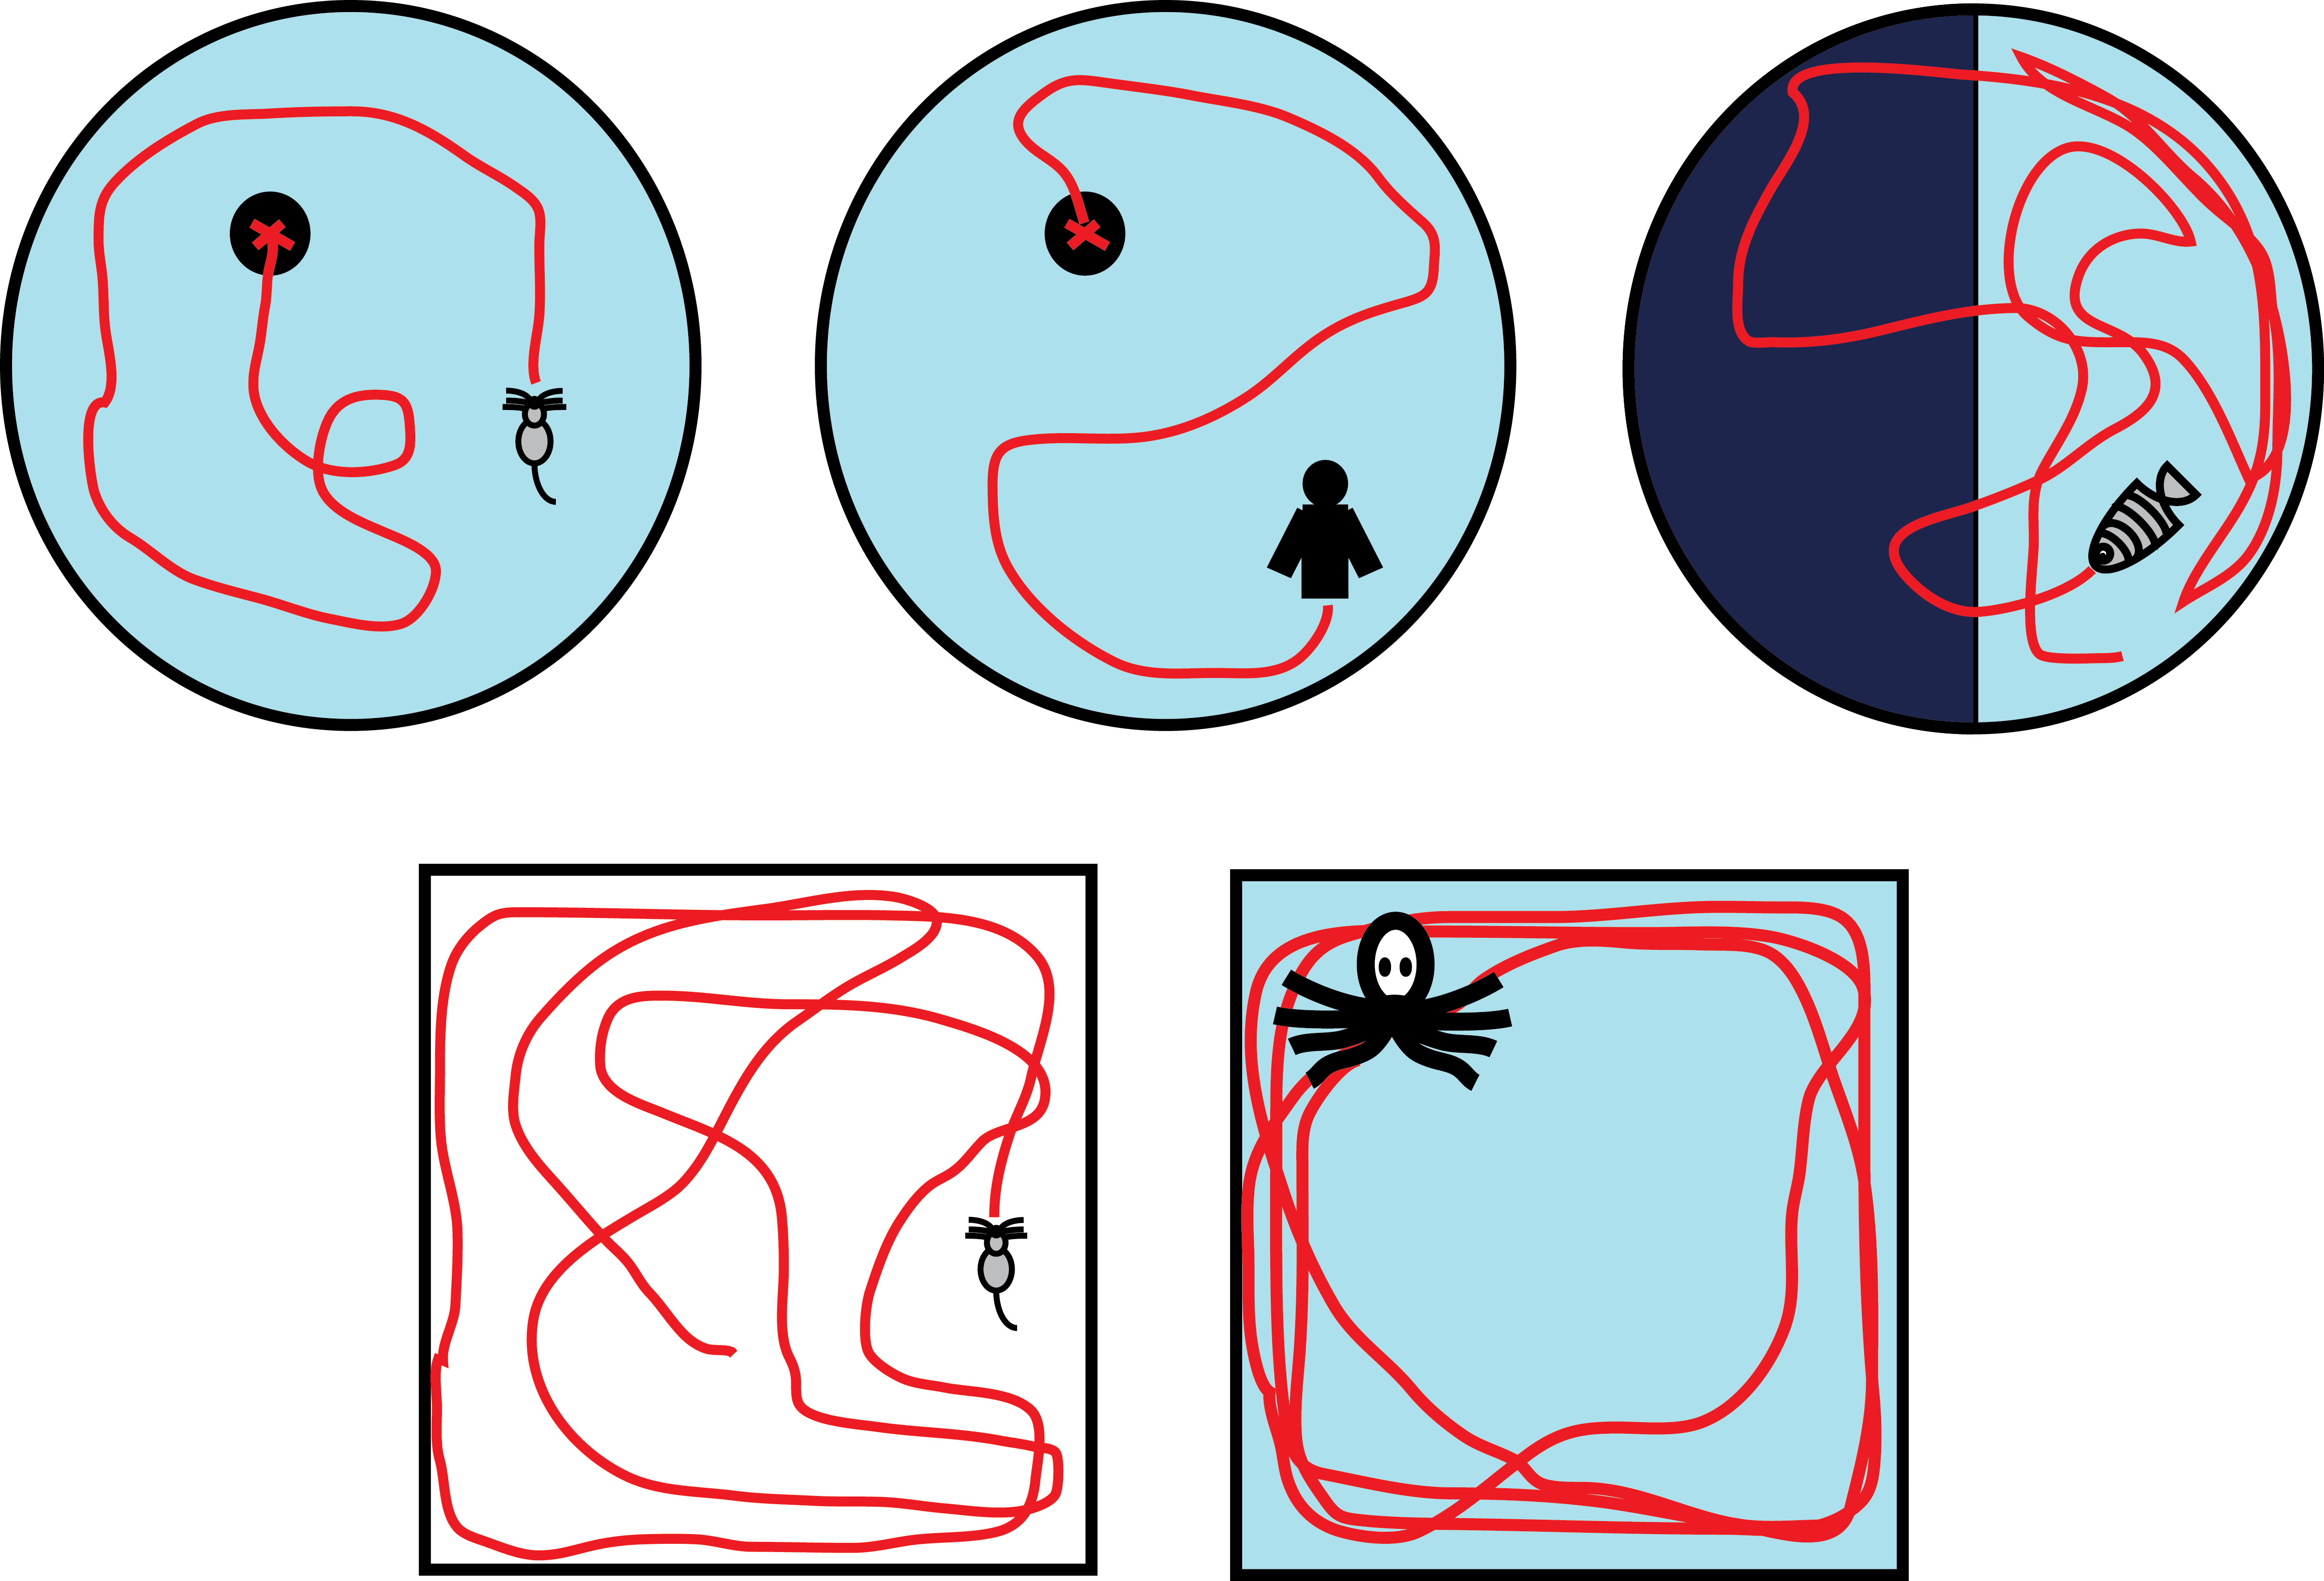
\includegraphics[width=0.47\textwidth]{figures/experiments}
	\end{figure}
	\vspace{0.05mm}
	\uncover<5->{
		\begin{itemize}[label={\MyShadow{$\bullet$}{red!80}}, leftmargin=*]
			\setlength\itemsep{0.01em}
			\item Limited to specific experiments.
			\item Require meta-parameter tuning.
			\item Crucial behavioural information might be lost.
		\end{itemize} 	
	}	
\end{multicols}
\end{frame}


\begin{frame}{The Morris Water Maze}
\begin{figure}[H]
	\centering
	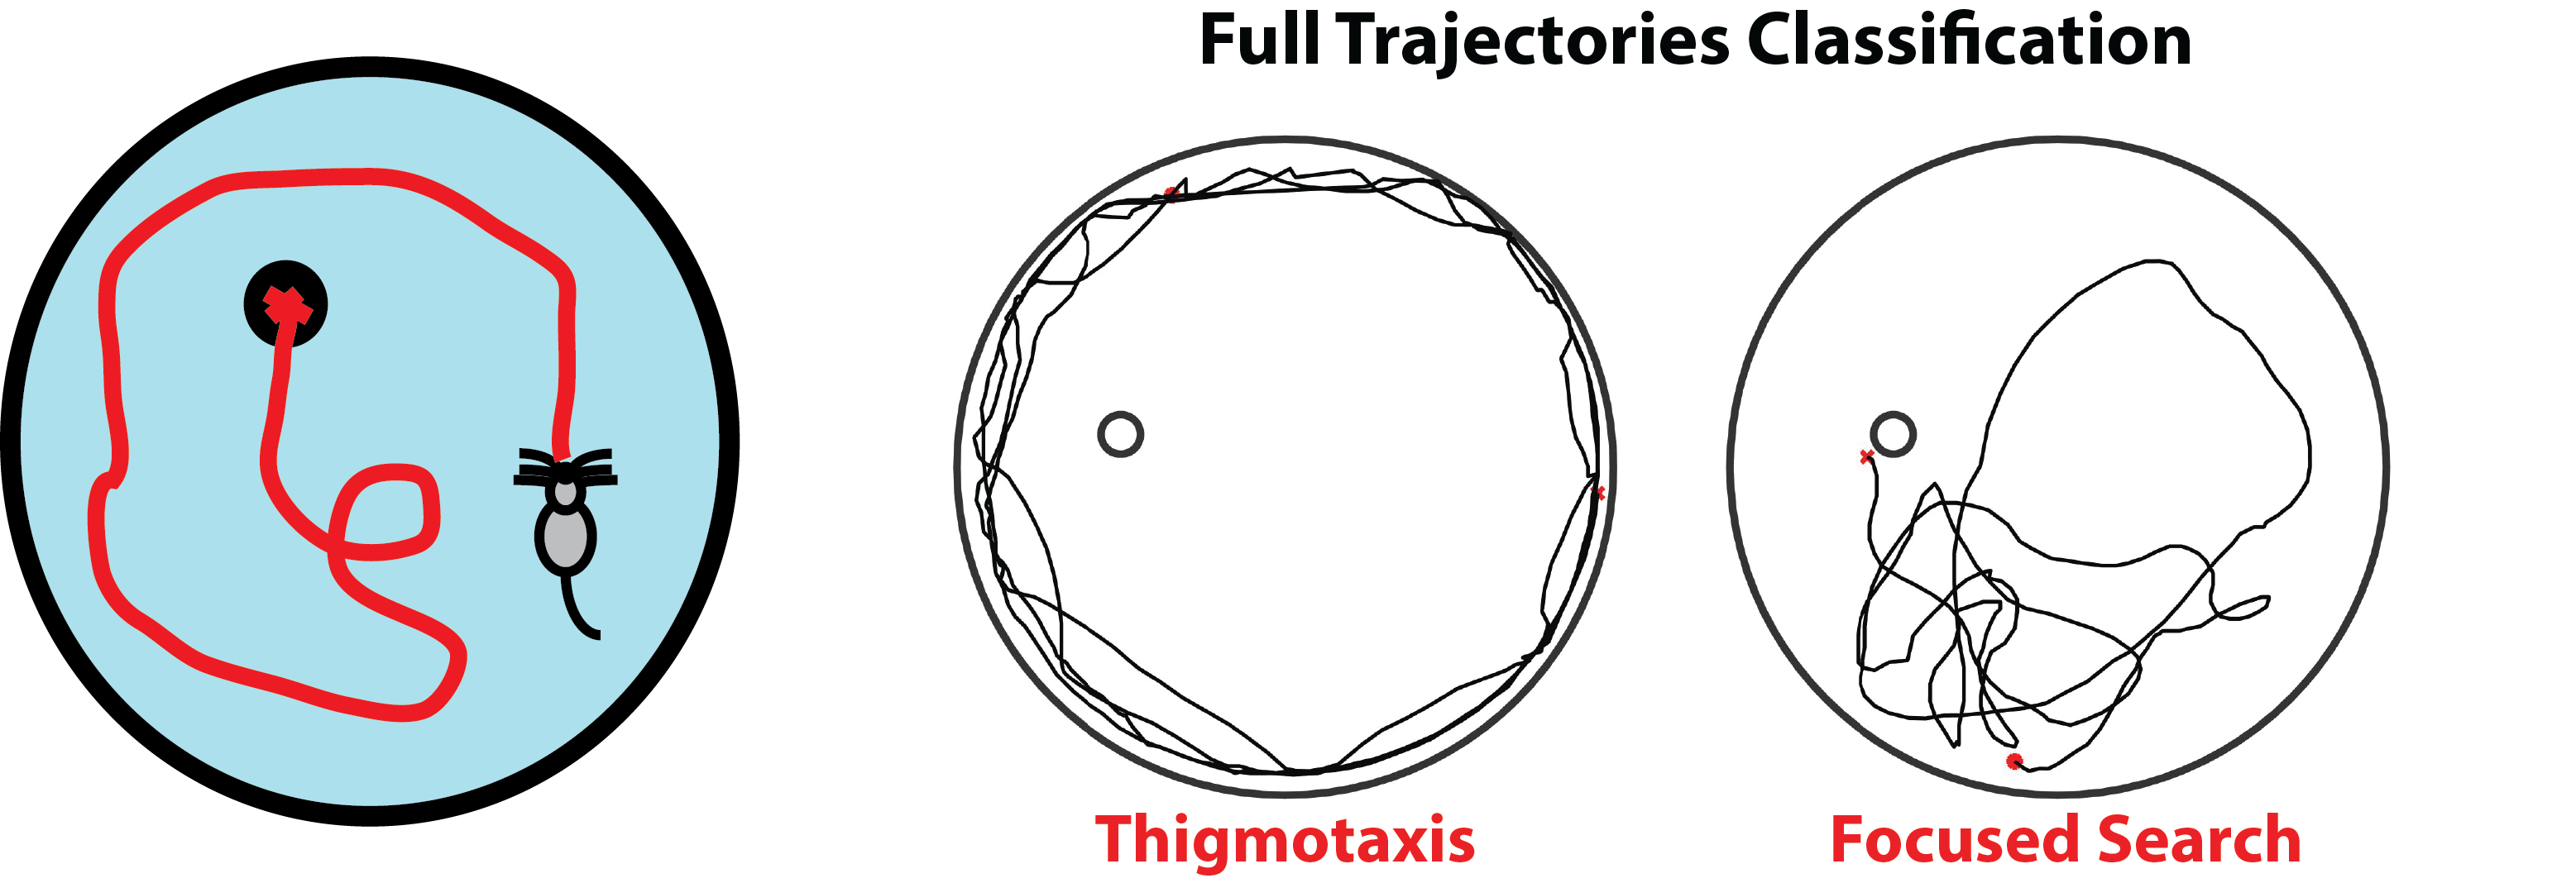
\includegraphics[width=0.9\textwidth]{figures/MWMothers}
\end{figure}	
\begin{multicols}{2}
	\small{
	\begin{itemize}[leftmargin=*]			
		\item
		\begin{itemize}[label={\MyShadow{$\bullet$}{blue!80}}]
			\item Dalm, S., Grootendorst, J., De Kloet, E. R. (2000).
			\vspace{1.2mm}	
			\item Wolfer, D. P. \& Lipp, H.-P. (2000).
			\vspace{1.2mm}
			\item Wolfer, D. P., Madani, R., Valenti, P. \& Lipp, H.-P. (2001).
			\vspace{1.2mm}
			\item Graziano, A., Petrosini, L. \& Bartoletti, A. (2003)
			\vspace{1.2mm}
			\item Illouz, T., Madar, R., Louzon, Y., Griffioen, K. J. \& Okun, E. (2016).
			\vspace{1.2mm}
			\item Rogers, Jake, et al. (2017).
			\vspace{1.2mm}
			\item Higaki, Akinori, et al. (2018).
		\end{itemize}		
	\end{itemize}
	}
\end{multicols}	
\end{frame}


\begin{frame}{The Morris Water Maze}
\begin{multicols}{2}
	\begin{itemize}[leftmargin=*]	
		\item<1->
			\vspace*{5mm}	
			\small{Gehring, T. V., Luksys, G., Sandi, C., \& Vasilaki, E. (2015).}
		\item<2->
			\vspace*{4mm}	
			\small{Vouros, A., Gehring, T. V., Szydlowska, K., Janusz, A., Tu, Z., Croucher, M., ... \& Vasilaki, E. (2018)}	
		\item<1->			
			\begin{figure}[H]
				\centering
				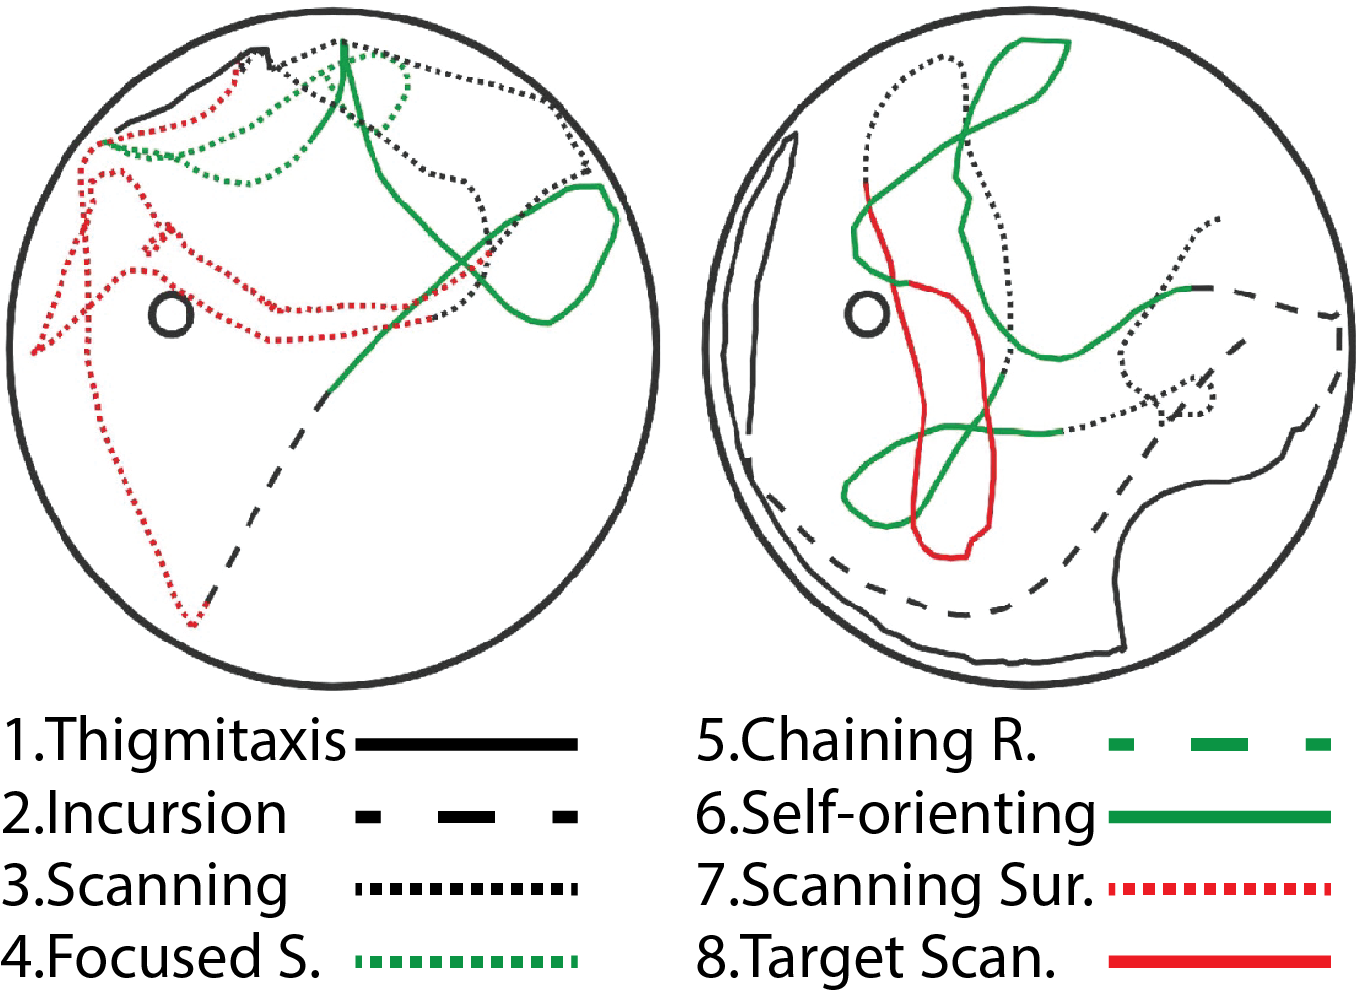
\includegraphics[width=0.40\textwidth]{figures/gehringetal}
			\end{figure}	
	\end{itemize}			
\end{multicols}		
\vspace{6mm}	
\begin{itemize}[leftmargin=*]
	\item<2->
	\begin{figure}[H]
		\centering
		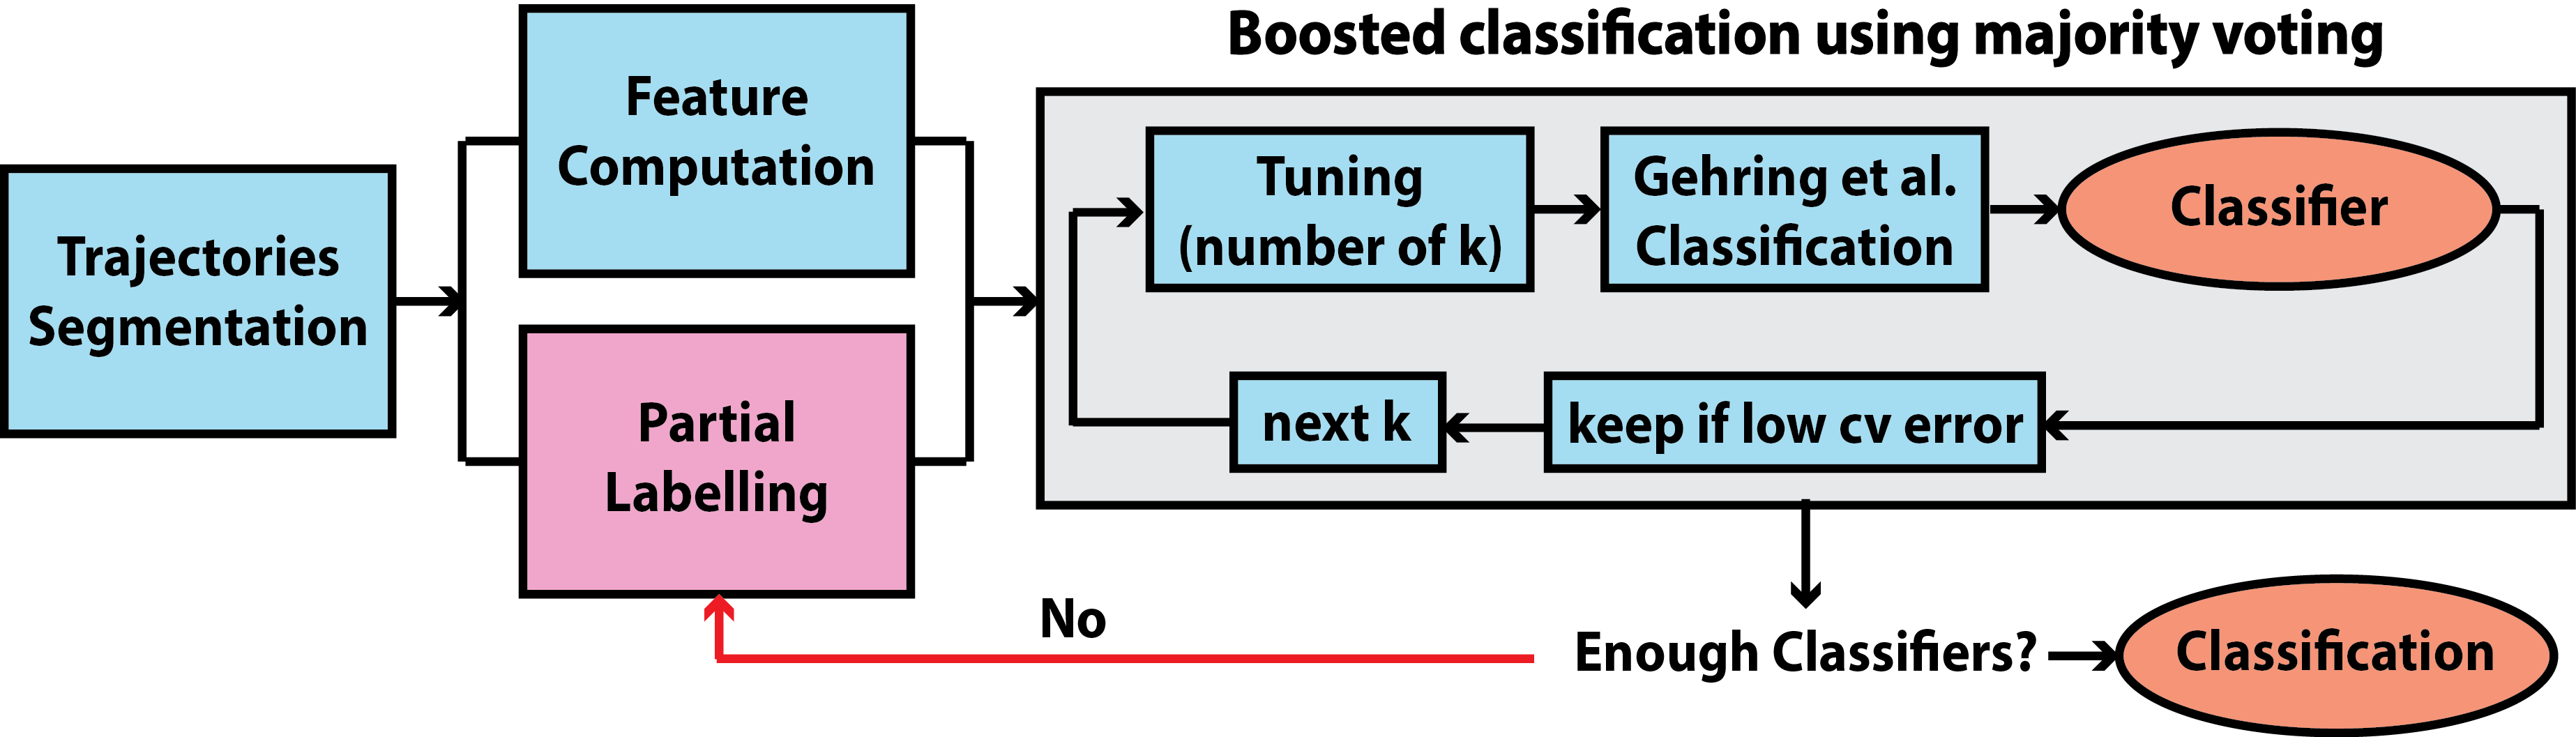
\includegraphics[width=0.90\textwidth]{figures/vourosetal}
	\end{figure}		
\end{itemize}	
\end{frame}


\begin{frame}{RODA collaborations}
	\begin{figure}[H]
		\centering
		
\includegraphics[width=\textwidth]{figures/roda}
	\end{figure}
\end{frame}
\begin{frame}{RODA collaborations}
	\begin{figure}[H]
		\centering
		
\includegraphics[width=\textwidth]{figures/collaborations1}
	\end{figure}		
\end{frame}
\begin{frame}{RODA collaborations}
	\begin{figure}[H]
		\centering
		
\includegraphics[width=\textwidth]{figures/collaborations2}
	\end{figure}		
\end{frame}


\begin{frame}{RODA collaborations}
	\begin{figure}[H]
		\centering
		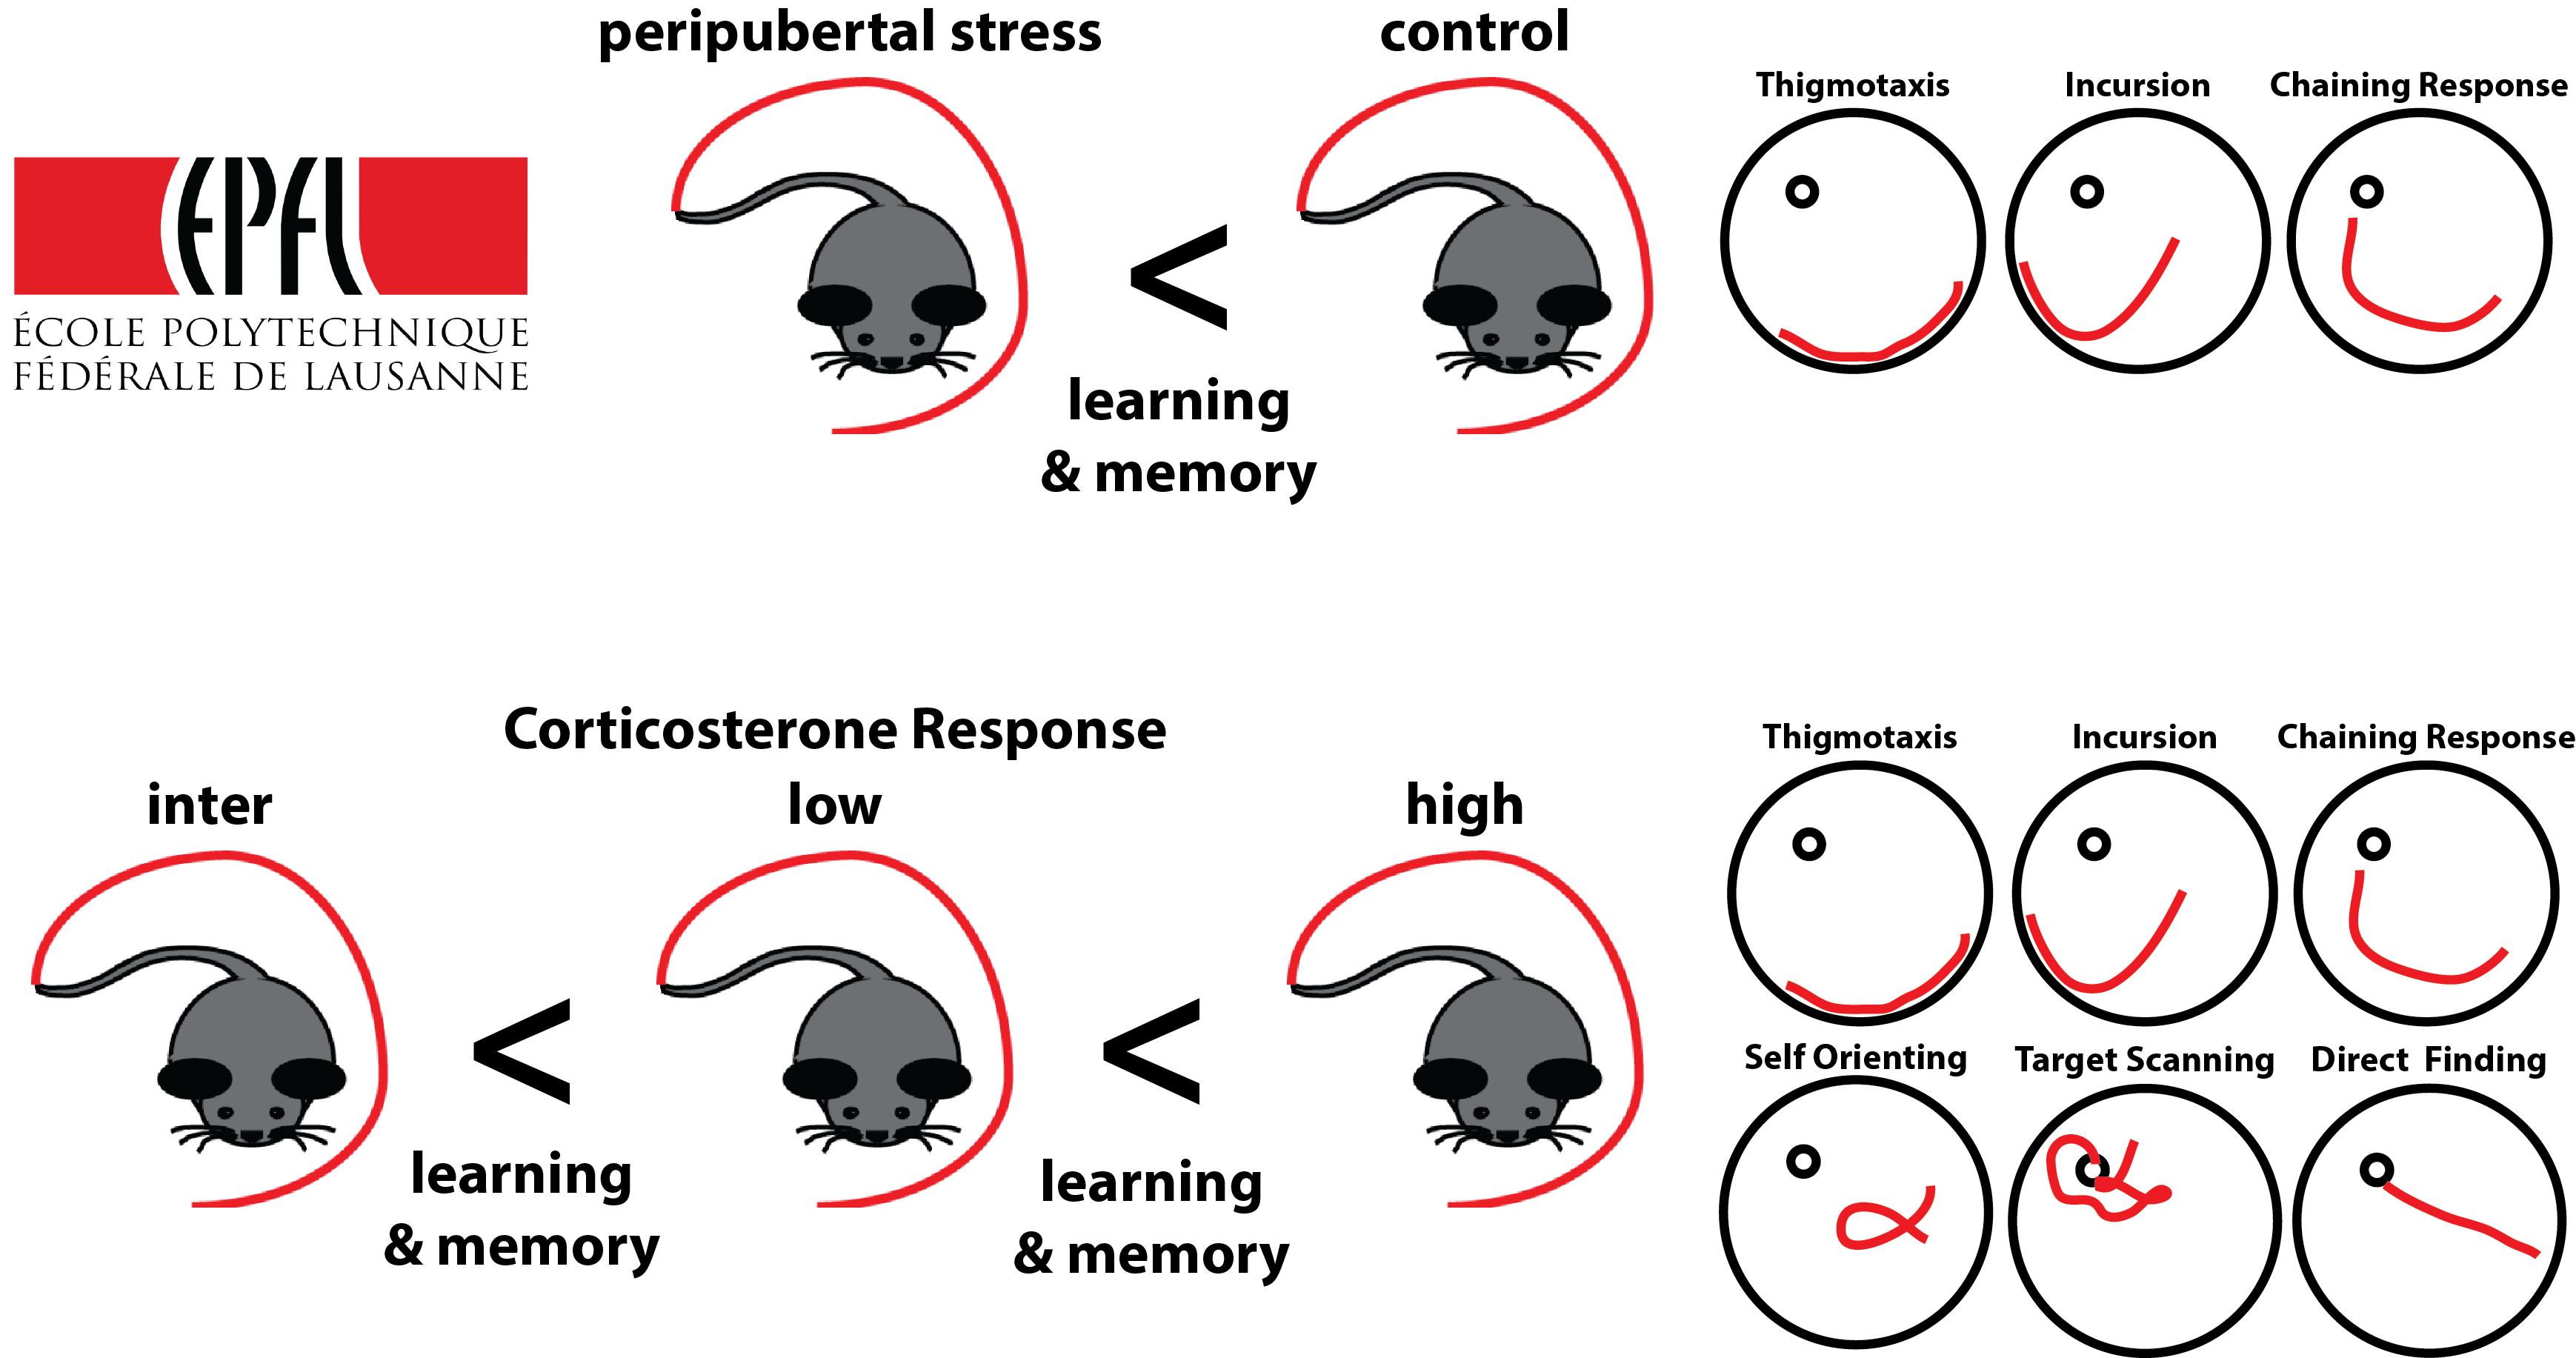
\includegraphics[width=\textwidth]{figures/EPFLwork}
	\end{figure}
	\begin{tiny}
		\begin{noindlist}
			\item Vouros, A., Gehring, T. V., Szydlowska, K., Janusz, A., Tu, Z., Croucher, M., ... \& Vasilaki, E. (2018). A generalised framework for detailed classification of swimming paths inside the Morris Water Maze. Scientific reports, 8(1), 15089.				
			\item Huzard, D., Vouros, A., Monari, S., Astori, S., Vasilaki, E., \& Sandi, C. (2019). Constitutive differences in glucocorticoid responsiveness are related to divergent spatial information processing abilities. bioRxiv, 579508. \textbf{Accepted $@$ Journal of Stress.}
		\end{noindlist}
	\end{tiny}	
\end{frame}


%----------------------------------------------


\begin{frame}{Unsupervised detection of behavioural motifs}
\begin{figure}[H]
	\centering
	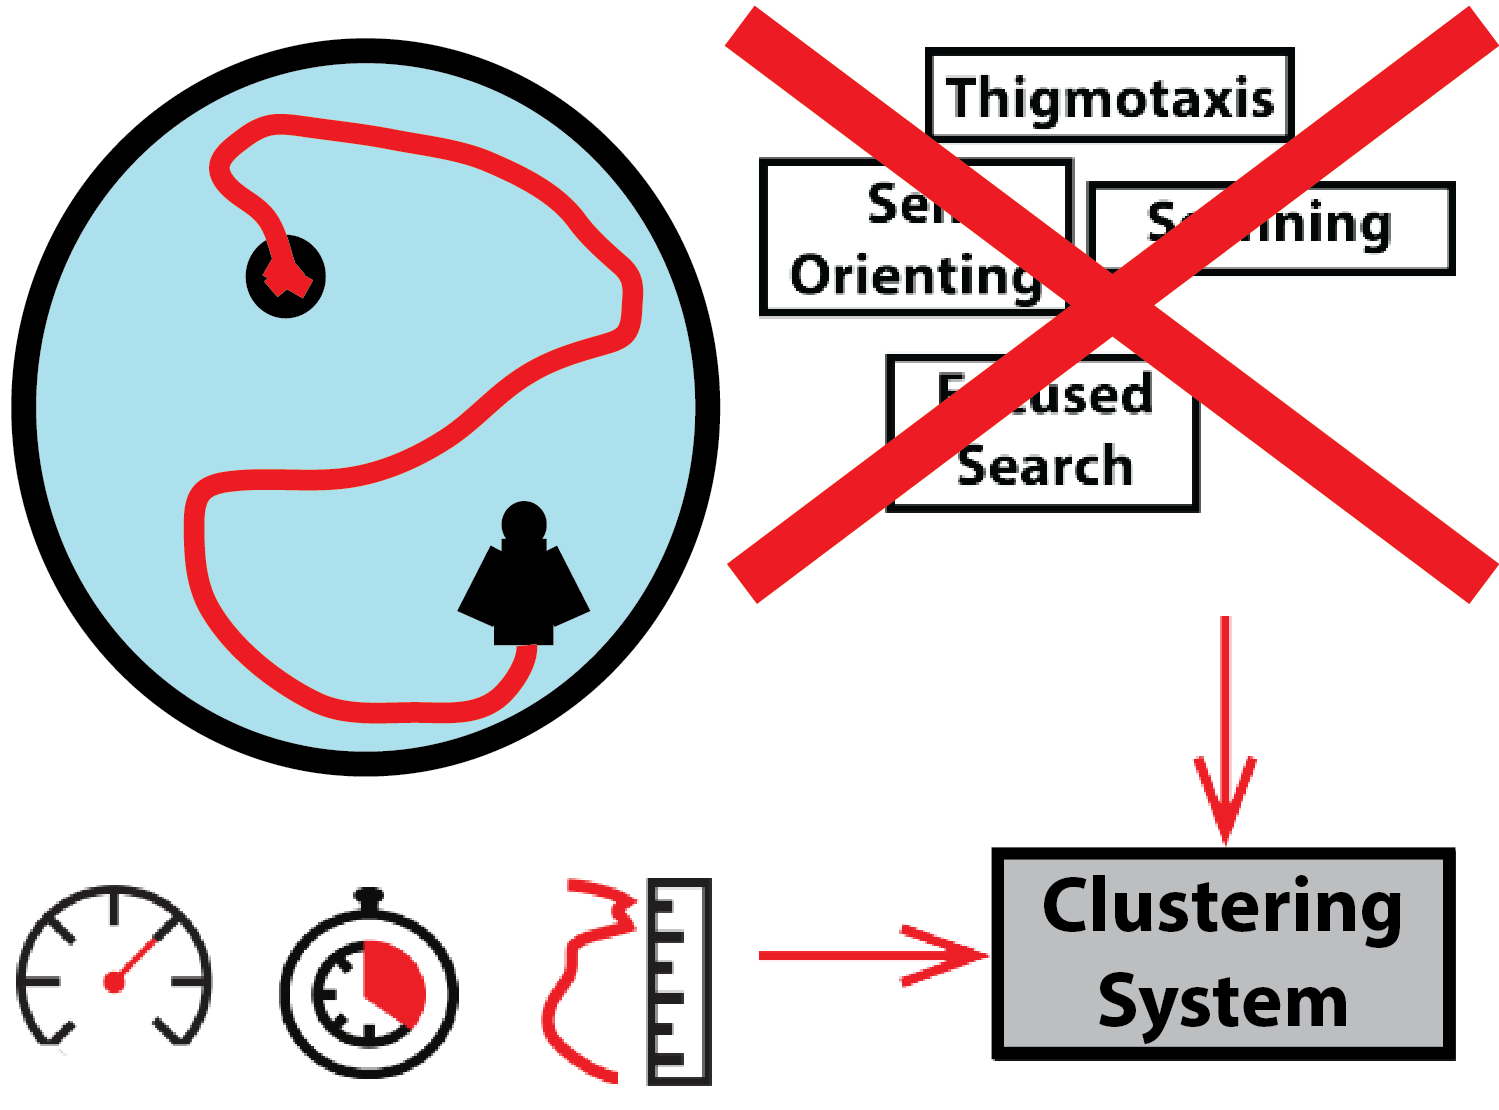
\includegraphics[width=0.7\textwidth]{figures/othersX3}
\end{figure}	
\end{frame}


\begin{frame}{Unsupervised detection of behavioural motifs}
\begin{figure}[H]
	\centering
	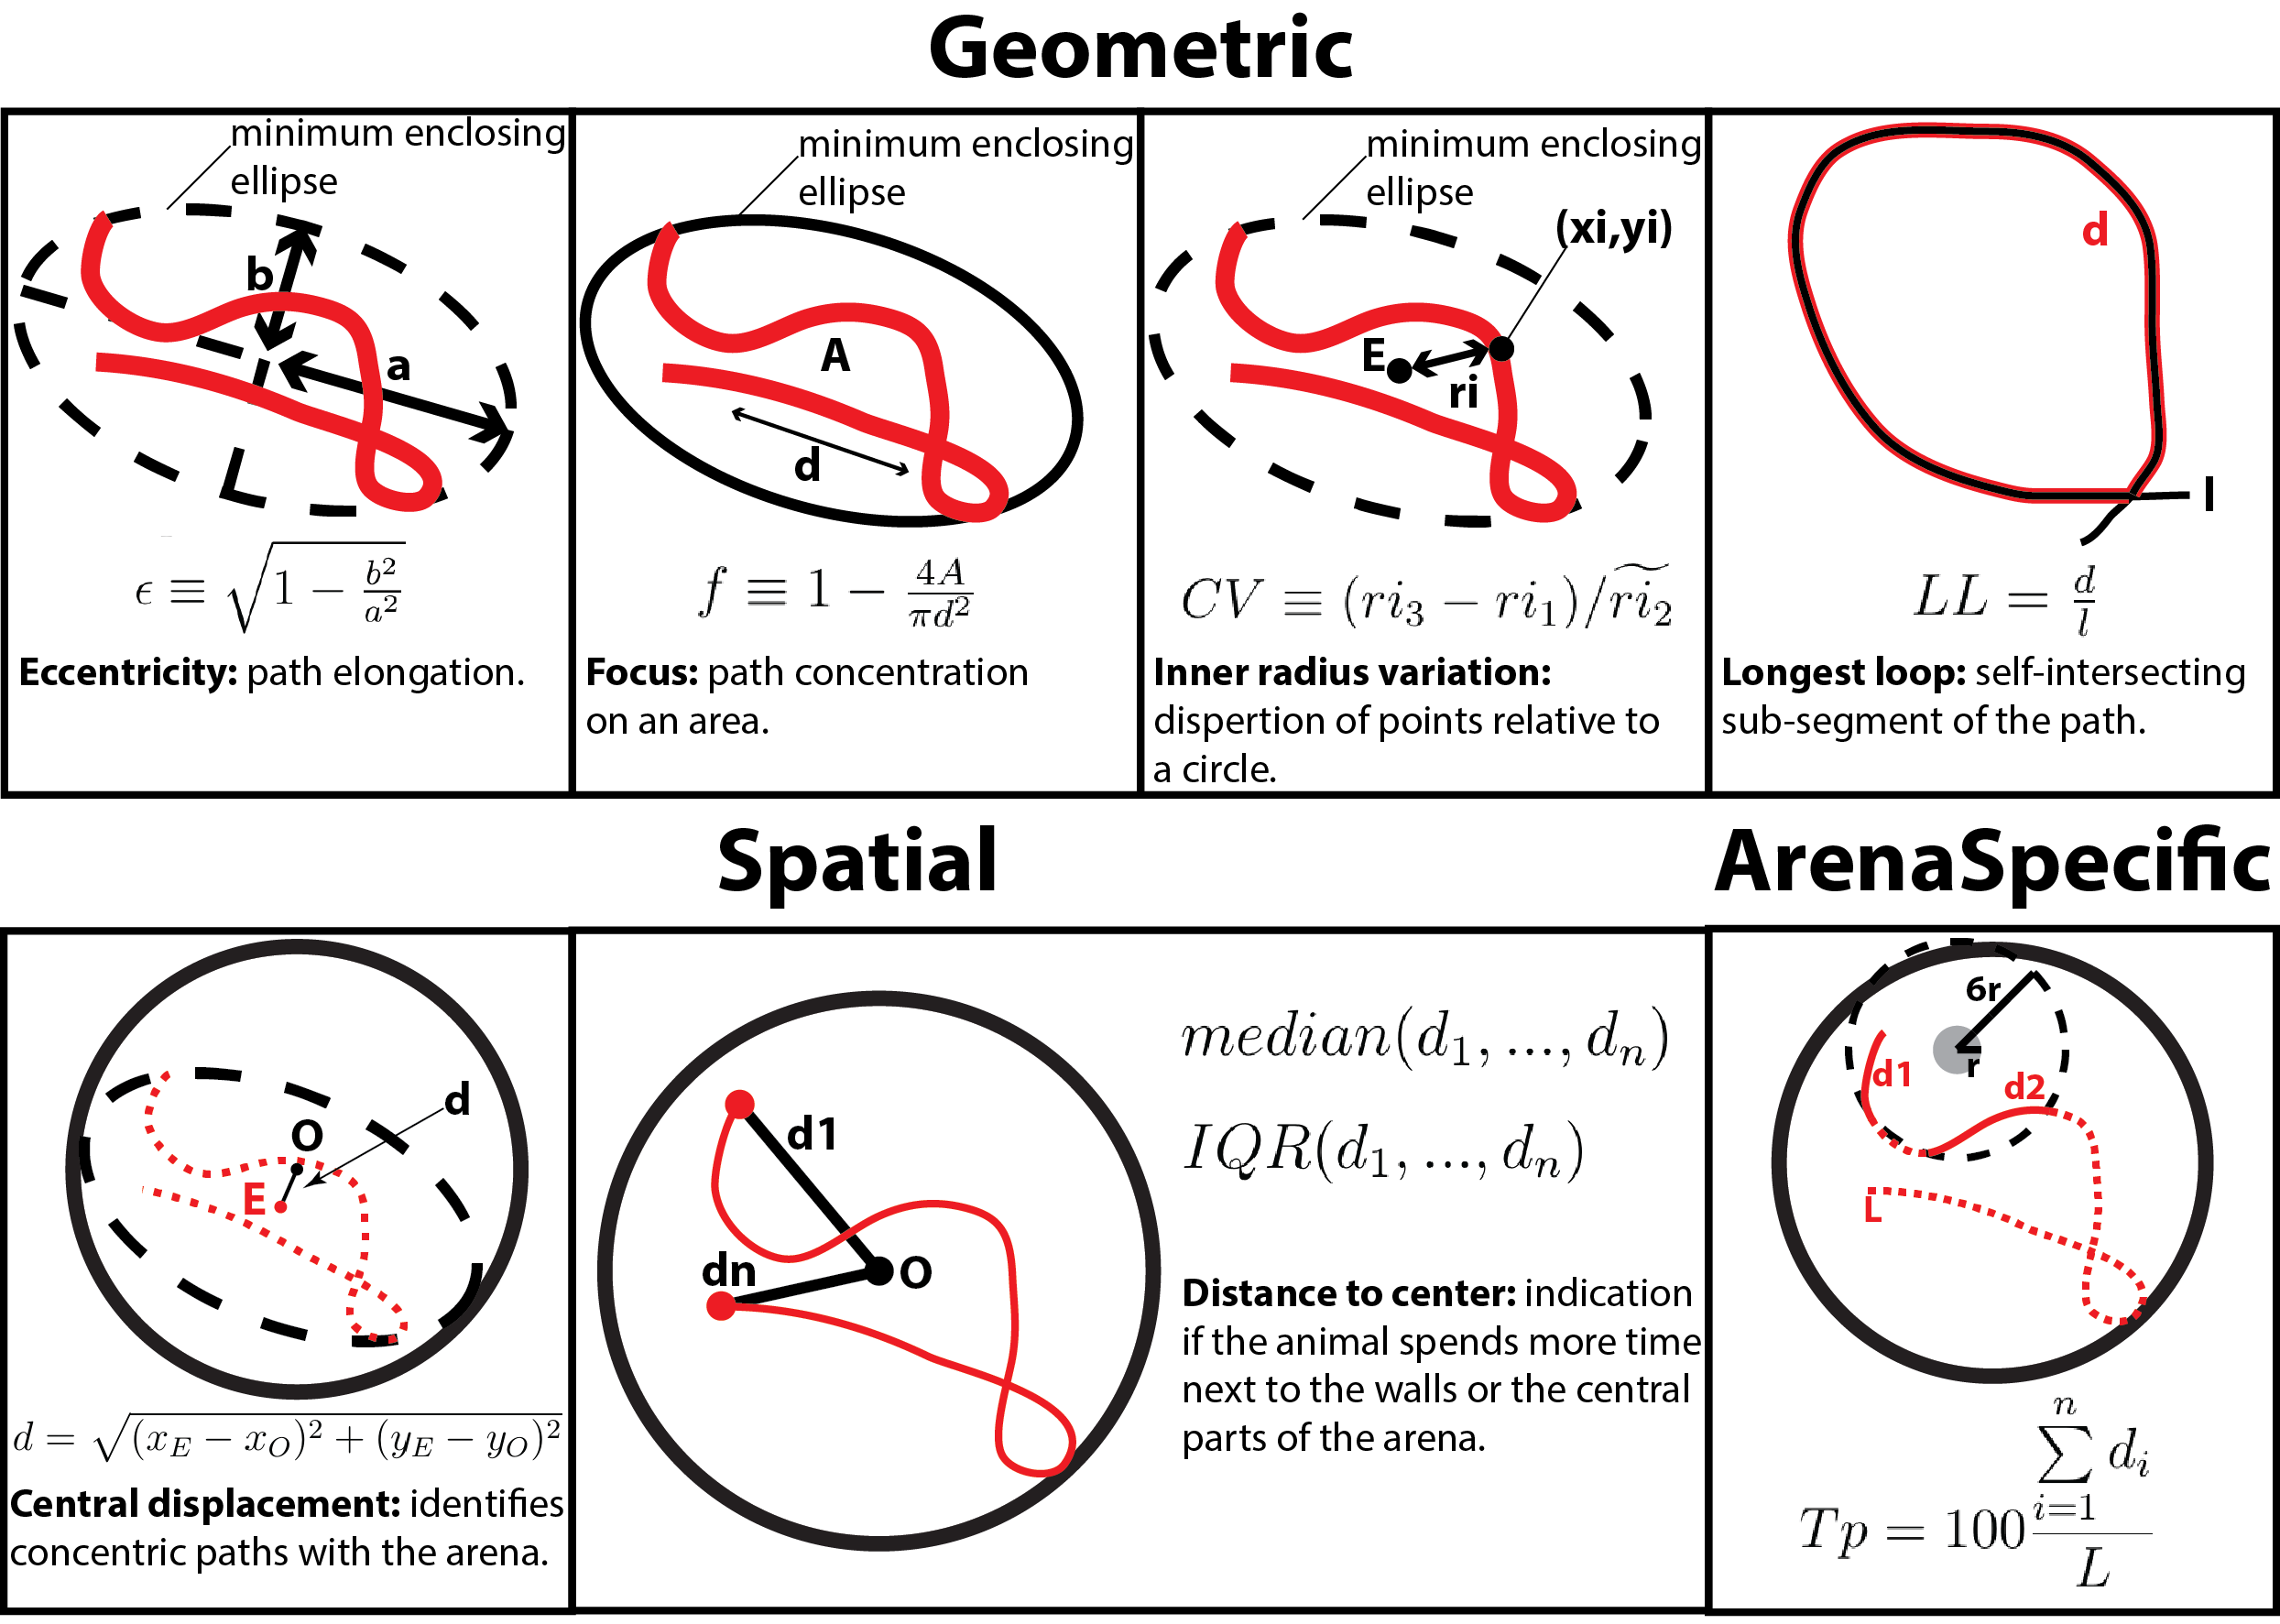
\includegraphics[width=0.7\textwidth]{figures/features}
\end{figure}
\begin{tiny}
	\begin{noindlist}	
		\item Gehring, T. V., Luksys, G., Sandi, C., \& Vasilaki, E. (2015). Detailed classification of swimming paths in the Morris Water Maze: multiple strategies within one trial. Scientific reports, 5, 14562.
		\item Vouros, A., Gehring, T. V., Szydlowska, K., Janusz, A., Tu, Z., Croucher, M., ... \& Vasilaki, E. (2018). A generalised framework for detailed classification of swimming paths inside the Morris Water Maze. Scientific reports, 8(1), 15089.
	\end{noindlist}	
\end{tiny}	
\end{frame}


\begin{frame}{Unsupervised detection of behavioural motifs}
\vspace{6mm}
\begin{figure}[H]
	\centering
	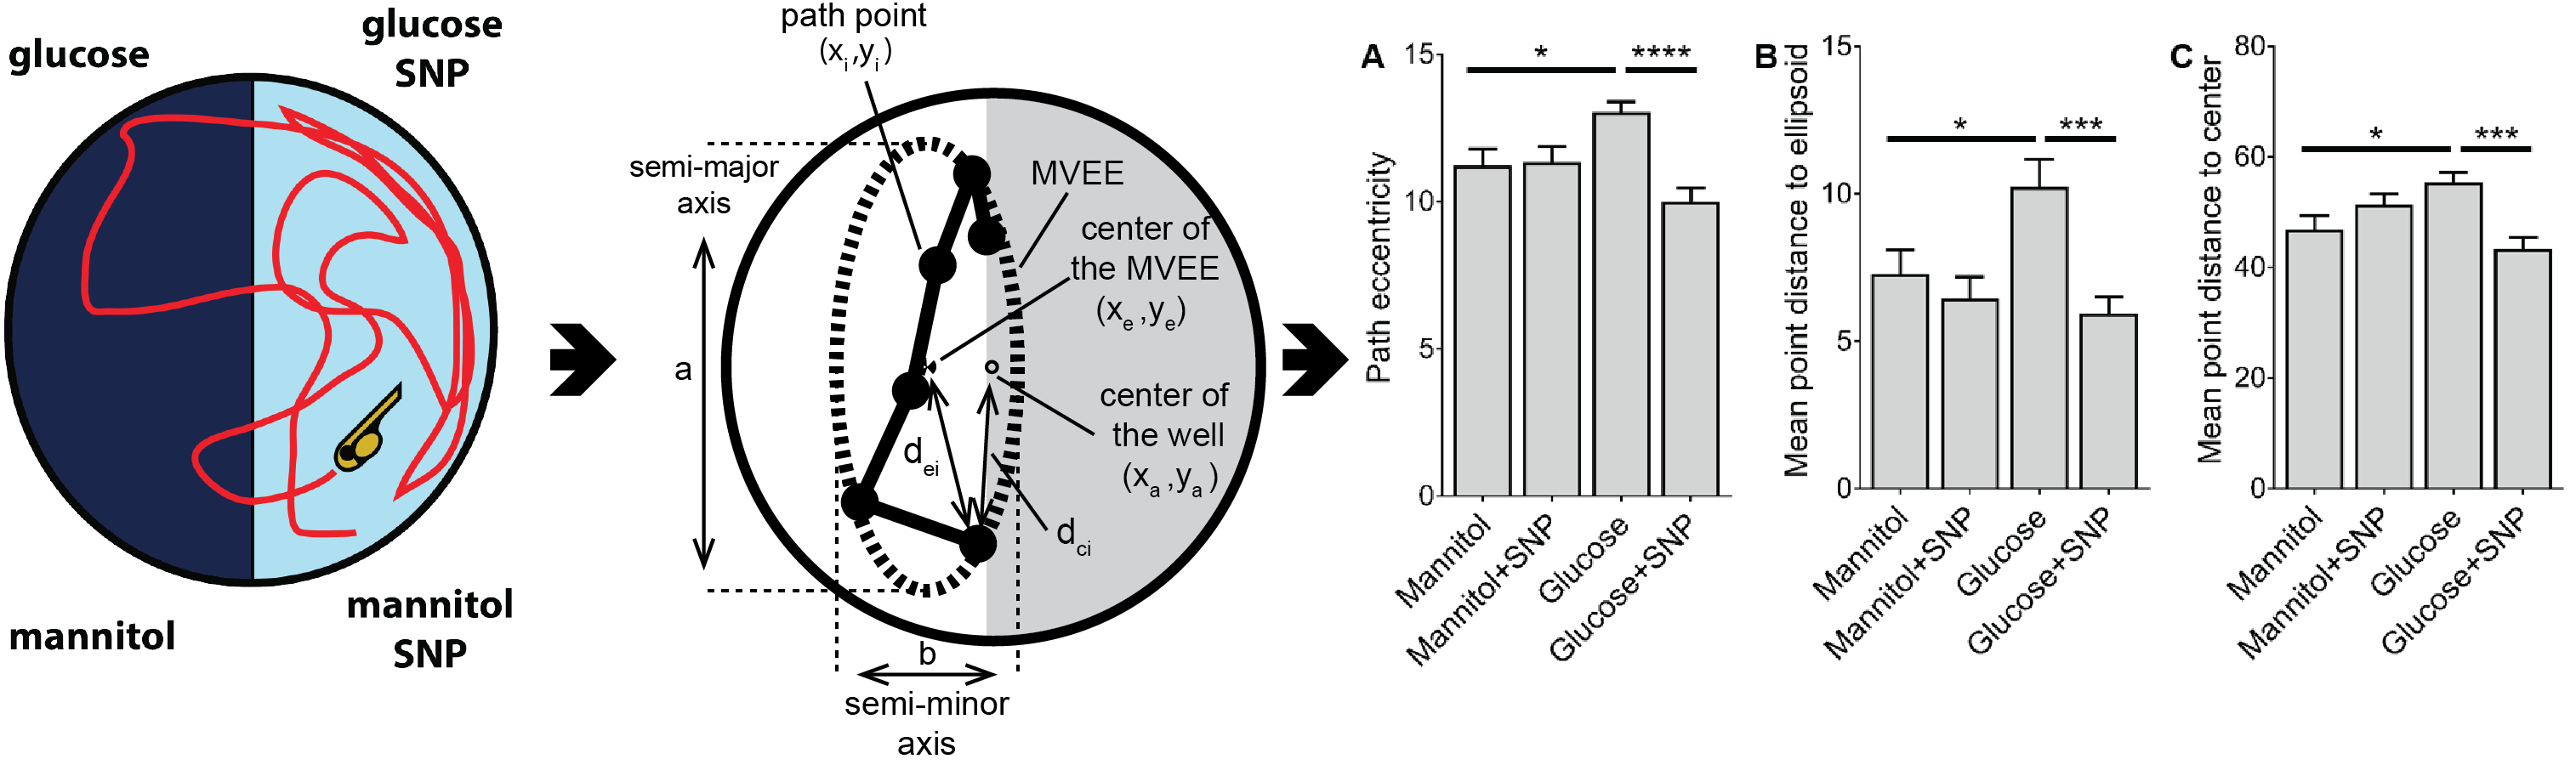
\includegraphics[width=\textwidth]{figures/karishmaetal}
\end{figure}
\vspace{16mm}
\begin{tiny}
	\begin{noindlist}	
		\item Chhabria, K., Vouros, A., Gray, C., MacDonald, R. B., Jiang, Z., Wilkinson, R. N., ... \& Chico, T. (2019). Sodium nitroprusside prevents the detrimental effects of glucose on the neurovascular unit and behaviour in zebrafish. bioRxiv, 576942. \\\textbf{Corrections $@$ Journal of Physiology.}
	\end{noindlist}	
\end{tiny}	
\end{frame}


\begin{frame}{Unsupervised detection of behavioural motifs}
\textbf{The K-Means Algorithm (Lloyd's)}
\begin{multicols}{2}
	\textbf{Advantages:}
	\begin{itemize}[label={\MyShadow{$\bullet$}{blue!80}}, leftmargin=*]
		\item Simple and easy to implement.
		\item Versatile.
		\item Guaranteed to converge. 
		\item Invariant to data ordering.			
	\end{itemize}
	\columnbreak 
	\textbf{Disadvantages:}
	\begin{itemize}[label={\MyShadow{$\bullet$}{red!80}}, leftmargin=*]
		\item Detects only spherical and well-separated clusters.
		\item Sensitive to noise and outliers (Euclidean).
		\item Converges to a local minimum. 			
	\end{itemize}			
\end{multicols}
\begin{itemize}[leftmargin=*]
	\item<2->
	\begin{tcolorbox}[colback=white!5,colframe=red]
	\begin{itemize}[leftmargin=*]
		\item \textbf{In general:}
	\end{itemize}
	\begin{itemize}[label={\MyShadow{$\bullet$}{green!80}}, leftmargin=*]
		\item Non-deterministic.	
		\item Sensitive to initial centroids location.
		\item Sensitive to features (variables/attributes).			
	\end{itemize}
	\end{tcolorbox}
\end{itemize}
\vspace{0.3cm}
\begin{itemize}[leftmargin=*]
	\item[]\tiny{Celebi, M. Emre, Hassan A. Kingravi, and Patricio A. Vela. ``A comparative study of efficient initialization methods for the k-means clustering algorithm.'' Expert systems with applications 40.1 (2013): 200-210.}	
\end{itemize}	
\end{frame}


\begin{frame}{Current work}
\begin{itemize}[leftmargin=*]
	\item
	\begin{itemize}[leftmargin=*]
		\item[{\MyShadow{$\bullet$}{blue!80}}]<1-> \textbf{Initialization: DK-Means++ [1] or D-ROBIN [2,3] method.} Make K-Means deterministic. 
		\item[{\MyShadow{$\bullet$}{blue!80}}]<2-> \textbf{Feature selection and assessment: Sparse K-Means [4].} Select informative features; weight them based on their clustering contribution.
		\item[{\MyShadow{$\bullet$}{red!80}}]<3-> \textbf{Automatic tuning:} Data driven meta-parameters tuning.
	\end{itemize}	
	\item<4->
	\begin{figure}[H]
		\centering
		
\includegraphics[width=0.6\textwidth]{figures/NAG2}
	\end{figure}
	\item
	\vspace{0.6cm}
	\begin{tiny}
		\begin{itemize}[leftmargin=*]
			\item[] $[1]$ Nidheesh, N., KA Abdul Nazeer, and P. M. Ameer. "An enhanced deterministic K-Means clustering algorithm for cancer subtype prediction from gene expression data." Computers in biology and medicine 91 (2017): 213-221.			
			\item[] $[2]$ Al Hasan, Mohammad, et al. "Robust partitional clustering by outlier and density insensitive seeding." Pattern Recognition Letters 30.11 (2009): 994-1002.
			\item[] $[3]$ Vouros, A., et al, \textbf{Manuscript under preparation.}	
			\item[]<2-> $[4]$ Witten, Daniela M., and Robert Tibshirani. ``A framework for feature selection in clustering.'' Journal of the American Statistical Association 105.490 (2010): 713-726.						
		\end{itemize}
	\end{tiny}		
\end{itemize}	
\end{frame}


\begin{frame}{Future research}
\textbf{Active Allothetic Place Avoidance task: \\The effects of silver nanoparticles on learning and memory. }
\begin{multicols}{2}
	\begin{figure}[H]
		\centering
		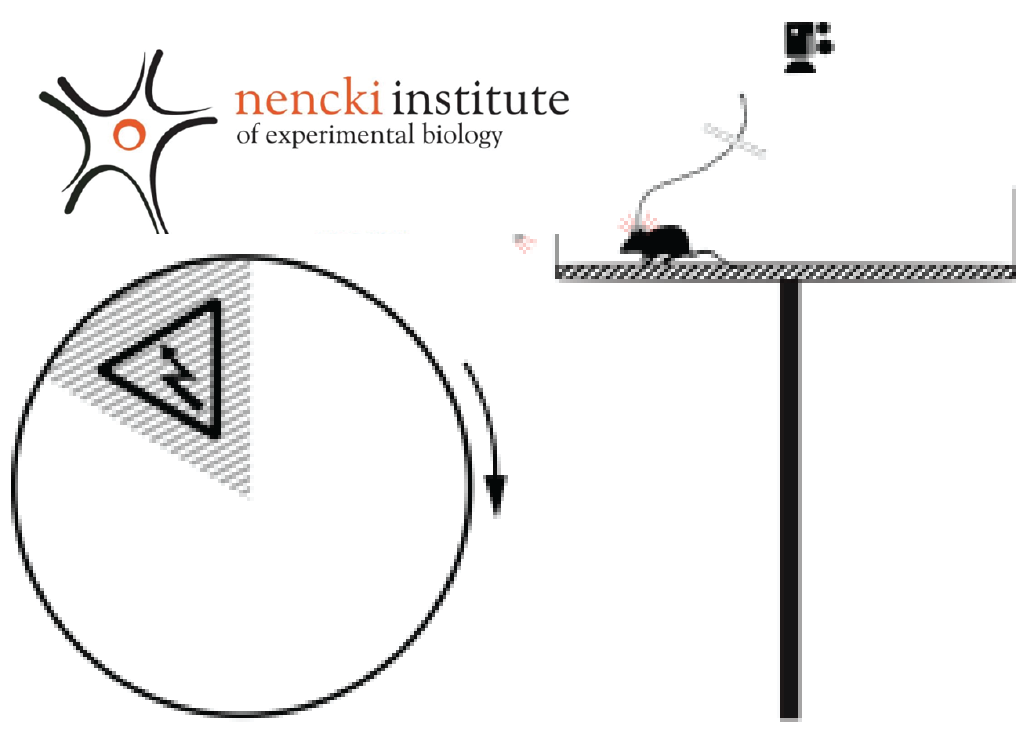
\includegraphics[width=0.5\textwidth]{figures/placeavoid2}
	\end{figure}
\begin{itemize}[label={\MyShadow{$\bullet$}{blue!80}}, leftmargin=*]
	\item[]<2-> 
	\item<2-> Detect and categorize animal behavioural motifs.
	\item<2-> Link behavioural motifs to different stages of learning and memory.
	\item<2-> Detect the dominant features of each motif.
\end{itemize}
\end{multicols}
\vspace{1.0cm}
\begin{tiny}
\begin{itemize}[leftmargin=*]
	\item[] Gehring, Tiago V., et al. ``Analysis of behaviour in the Active Allothetic Place Avoidance task based on cluster analysis of the rat movement motifs.'' bioRxiv (2017): 157859.	
\end{itemize}
\end{tiny}	
\end{frame}


\begin{frame}[plain,c]
\begin{Large}
	\begin{center}
		\textbf{Thank you for your attention!}
	\end{center}
\end{Large}	
\begin{figure}[H]
	\centering
	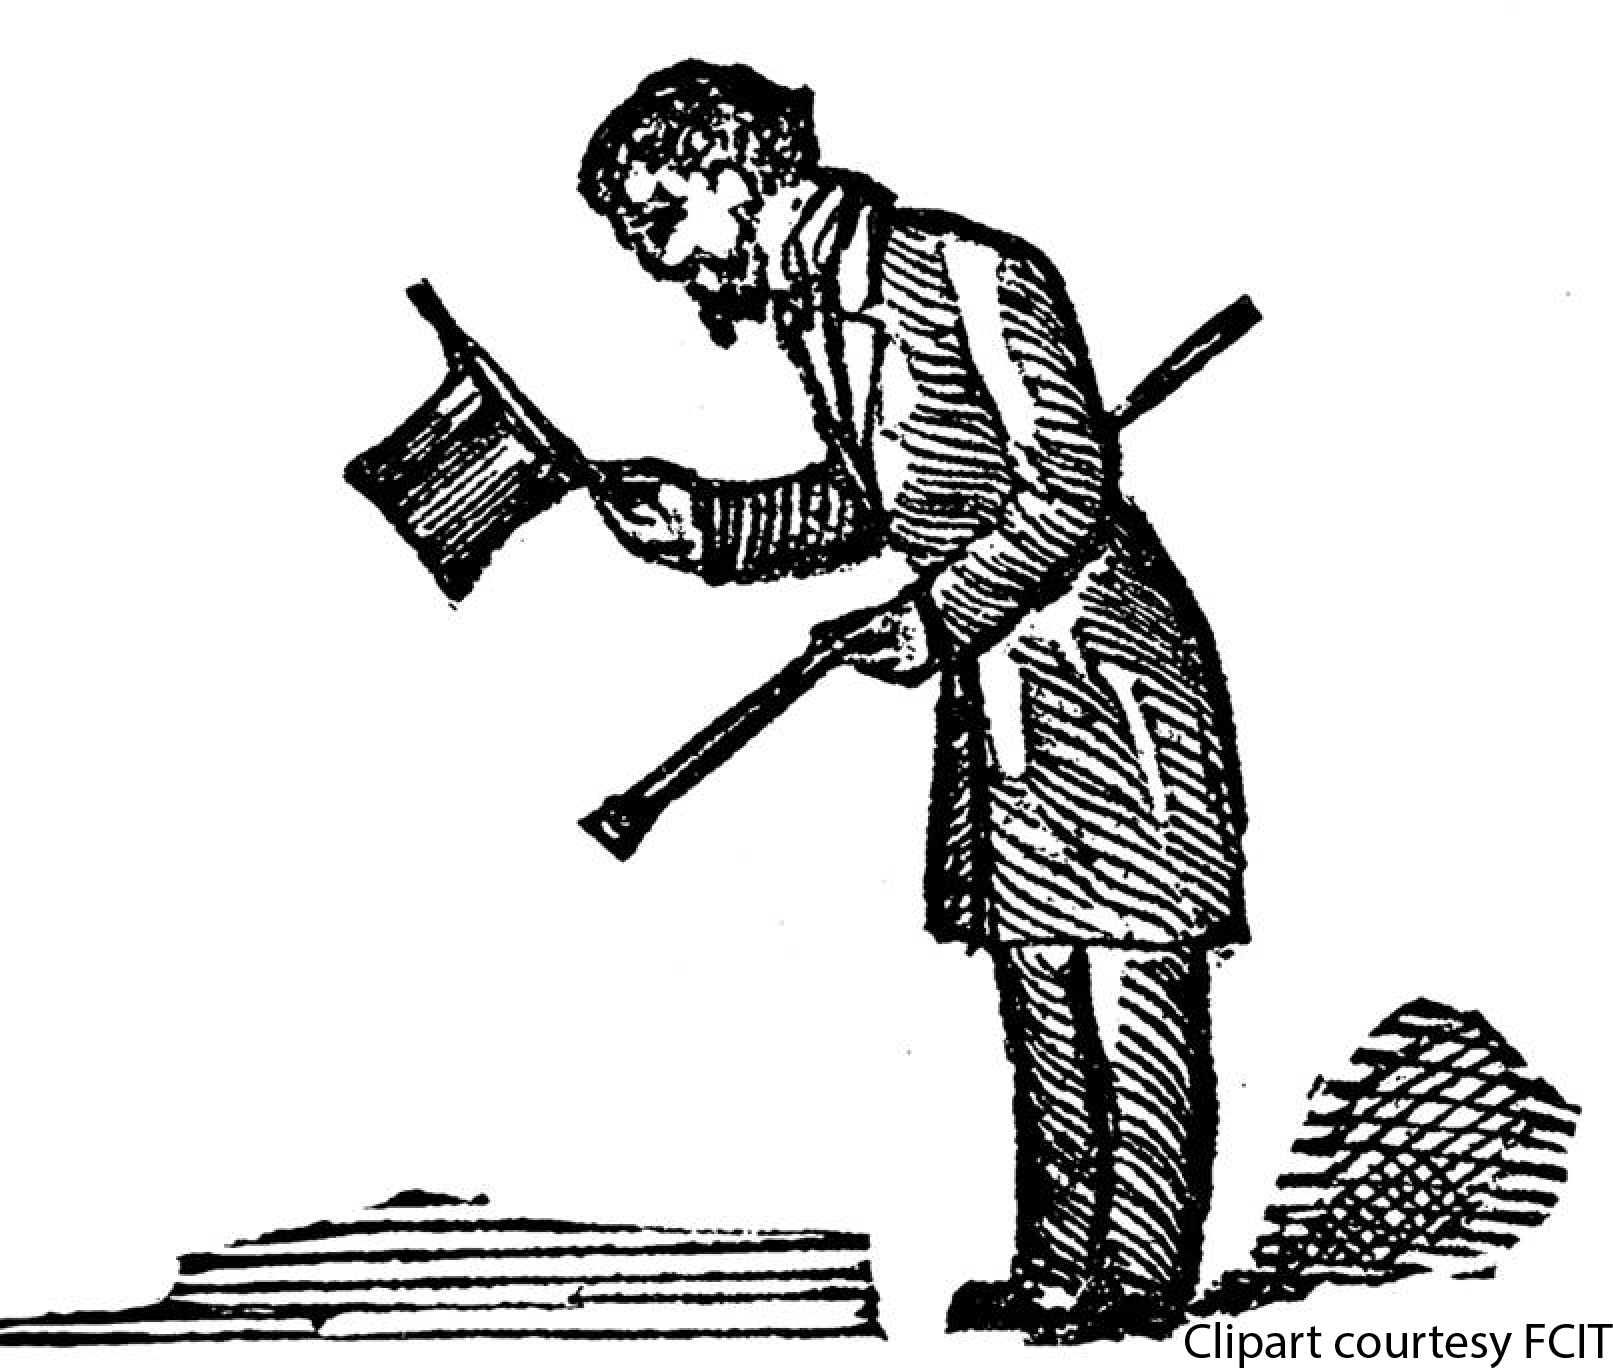
\includegraphics[width=0.5\textwidth]{figures/final}
\end{figure}
\end{frame}


}
\end{document}

